\documentclass[a4paper,11pt]{article}
%Use article for short documents
\usepackage[T1]{fontenc}
\usepackage{parskip}
\usepackage{latexsym,amsmath,amssymb}
\usepackage{natbib}
\usepackage{graphicx}
\usepackage{times}
\usepackage{zi4}
\usepackage[a4paper,left=3cm,right=3cm,top=3cm,bottom=3cm]{geometry}

\title{The title}
\author{Jesse Murray}

\begin{document}
\maketitle
\thispagestyle{empty}
\newpage
\pagenumbering{arabic}

\section{Introduction}
This is an introduction section.
Some characters need to be typset carefully, for example \%, \# and \$.

\section{Model}

\subsection{Conceptual basis}
The conceptual idea behind the model is that the polygenic score of an offspring is expected be similar the parent value, but regress towards the mean with expecation regression coefficient $r$. There will also be random variation around that expected value such that the variance of the offspring's polygenic score is the variance of the parent's generation scaled by $r_s$.

The analogy of polygenic scores is used because polygenic scores are theorized to be normally distributed by the central limit theorem - as they are the sum of many (*poly*) genes, which are largely independent and whose effect can have any distribution, e.g., Bernoulli, Uniform, Normal, etc.

\subsection{Initial conditions and transitions}
The Markov chain exists in discrete time $\{0, 1, 2,...\}$, representing generations; and continuous space $\mathbb{R}$, representing polygenic scores.

Let all $Z$ be independent and identically distributed (i.i.d.) as $\mathcal{N}(0, 1)$.

Define the initial condition such that $X_0 \sim \mathcal{N}(0, \sigma_0^2)$:

$$X_0 = \sigma_0 Z$$

Define the one-step relationship between past and present states:

$$X_n = \tilde{\mu}_n + \epsilon$$

Such that:

$$\tilde{\mu}_n = rX_{n-1}, \qquad \epsilon = \tilde{\sigma}_n Z, \qquad \tilde{\sigma}_n = r_s \sigma_{n-1}$$

Rewriting the one-step relationship with these quantities we have:

$$X_n = rX_{n-1} + r_s \sigma_{n-1}Z$$

\subsection{The random state for any generation $n$.}

It can be shown by induction and the theorem of the sum of independent normal distributions that $X_n \sim \mathcal{N}(0, \sigma_n^2)$:

$$X_n = \sigma_n Z$$

Additionally, for $n > 0$ and $Z_a$, $Z_b$ independent standard normal random variables:

$$X_n = r\sigma_{n-1}Z_a + r_s\sigma_{n-1}Z_b$$



\subsection{The variance for any generation $n$.}
It follows immediately that $\sigma_n^2$ has the following one-step relationship:

$\sigma_n^2 = \sigma_{n-1}^2(r^2+r_s^2)$

By induction, $\sigma_n^2$ can also be stated in terms of the initial variance:

$\sigma_n^2 = \sigma_{0}^2(r^2+r_s^2)^n$


\section{Properties}

\subsection{Variance of $\epsilon$}

$$\tilde{\sigma}_n = r_s (r^2+r_s^2)^{\frac{n-1}{2}} \sigma_0$$


\subsection{The conditional expectation for any generation $n$}

$$\mathrm{E}(X_n|X_0) = r^nX_0$$


\subsection{Other Properties}

$$X_n|X_{n-1} \sim \mathcal{N}(\tilde{\mu}_n, \tilde{\sigma}_n^2)$$


$$\mathrm{Cov}(X_n, X_{n-1}) = r \sigma_{n-1}^2$$

$$\mathrm{Corr}(X_n, X_{n-1}) = r \frac{\sigma_{n-1}}{\sigma_n}$$


\section{Stable population variance}
Let a stable population variance be defined as follows:

$$\sigma_n^2 = \sigma_{n-1}^2$$

The following are a few important properties that occur under stable population variance:

$$r^2+r_s^2 = 1$$

$$\mathrm{Corr}(X_n, X_{n-1}) = r$$

For an aribrary state $i$:

$$\sigma_i^2 = \sigma_{0}^2$$




\section{Transition kernel}

Let $A$ be a subset of the state space:

$$A \subseteq \mathbb{R}$$

\subsection{State to set}
Then the transition kernel $P(A, x_{n-1})$ gives the one-step probability of reaching the set $A$ from the state $x_{n-1}$. 

$$P(A, x_{n-1}) = \int_{x_n\in A}^{} f(x_n|x_{n-1})f(x_{n-1}) \, dx_{n}$$

Where $f(x_n|x_{n-1})$ is the conditional probability density function (pdf) of $X_n|X_{n-1} \sim \mathcal{N}(\tilde{\mu}_n, \tilde{\sigma}_n^2)$, and $f(x_{n-1})$ is the pdf of $X_{n-1} \sim \mathcal{N}(0, \sigma_{n-1}^2)$.

\subsection{Set to set}
A similar transition kernel $P(A, B)$ can be used to obtain the one-step probability of reaching the set $A$ from the set $B$. 

$$B \subseteq \mathbb{R}$$

$$P(A, B) = \int_{x_{n-1}\in B}^{} P(A, x_{n-1}) \, dx_{n-1}$$

\subsection{Probability attributable}
Define the probability that a current state $X_n$ in set $A$ resulted from or is 'attributable' to a previous state or parent score $X_{n-1}$ in set $B$.

$$\large P_{\alpha}(A, B) = \frac{P(A, B)}{P(A, \mathbb{R})}$$

By the law of total probability, $P(A, \mathbb{R})$ is the marginal probability that the state $X_n$ is in the space $A$, which is given by $P(A)$:

$$P(A) = \int_{x_n\in A} f(x_n) \, dx_{n}$$

Therefore:

$$P_{\alpha}(A, B) = \frac{P(A, B)}{P(A)}$$




\subsection{Probability destined}
Define the probability that a previous state $X_{n-1}$ in set $B$ will result in or is 'destined' for a current state or offspring score $X_n$ in set $A$. 

$$P_{\delta}(A, B) = \frac{P(A, B)}{P(\mathbb{R}, B)}$$

Because the integral over the entire support of a pdf equals 1, $P(\mathbb{R}, B)$ is the marginal probability that the state $X_{n-1}$ is in the space $B$, which is given by $P(B)$:

$$P(B) = \int_{x_n\in B} f(x_{n-1}) \, dx_{n-1}$$



Therefore:

$$P_{\delta}(A, B) = \frac{P(A, B)}{P(B)}$$


\section{Linear regression}
$$\mathrm{E}(X_n|X_{n-1}) = rX_{n-1}$$

$$X_n = rX_{n-1} + \epsilon$$





This has the same form as the linear regression model where $b$ can be estimated by minimising the sum of the squared errors.

$$\mathrm{E}(Y|X) = bX$$

$$Y = bX + \epsilon$$

This means we can estimate $r$ through the least-squares approach. 






\section{Reverse one-step transition}
The parent's phenotypic score is also a random variable that is dependent on the offspring's phenotypic score. 

$$X_{n-1} = \frac{1}{r}X_n + \frac{r_s}{r}\sigma_{n-1}Z$$


$$X_{n-1}|X_{n} \sim \mathcal{N}(\frac{1}{r}X_n, \frac{r_s^2}{r^2}\sigma_{n-1}^2)$$


Where the variance can be rewritten in terms of the $n$th generation's variance:

$$\mathrm{Var}(X_{n-1}|X_{n}) = \frac{r_s^2}{r^2(r^2+r_s^2)} \sigma_n^2$$

\section{Eve's law}
It is possible to compute $\mathrm{Var(X_n)}$ through Eve's law:

$$\mathrm{Var(X_n)} = \mathrm{E}(\mathrm{Var}(X_{n-1}|X_n)) + \mathrm{Var}(\mathrm{E}(X_n|X_{n-1}))$$

We have that:

$$X_n = rX_{n-1} + \tilde{\sigma}_n Z$$

$$\tilde{\sigma}_n = r_s \sigma_{n-1}$$

Therefore, each term in Eve's law is:

$$\mathrm{E}(\mathrm{Var}(X_{n}|X_{n-1})) = \mathrm{E}(r_s^2 \sigma_{n-1}^2) = r_s^2 \sigma_{n-1}^2$$

$$\mathrm{Var}(\mathrm{E}(X_n|X_{n-1})) = \mathrm{Var}(rX_{n-1}) = r^2\sigma_{n-1}^2$$

Combining these terms, we confirm the variance of $X_n$:

$$\mathrm{Var(X_n)} = \sigma_{n-1}^2(r^2 + r_s^2)$$









\section{Use cases}
With the two parameters $r$ and $r_s$, we can perfectly describe the variance of the offspring's generation relative to that of the parent's generation through the following relation:

$$\frac{\sigma_n^2}{\sigma_{n-1}^2} = r^2+r_s^2$$

Simply knowing or having measured two of the three values: the ratio parent generation and offspring generation variance, the expectation regression coefficient ($r$), the standard deviation scaling coefficient ($r_s$); it is possible to obtain the third.

This can be useful, for example, to obtain the standard deviation of the offspring's polygenic score, after having measured the parent's polygenic score: $\tilde{\sigma}_n = r_s \sigma_{n-1}$.

Alternatively, after having only measured the $\frac{\sigma_n^2}{\sigma_{n-1}^2}$, which is 1 when there is stable population variance, and $r$, which can be obtained through ordinary least squares with the parent and offspring data or by the correlation coefficient between parent and offspring when there is stable population variance; the model can be constructed and applied.




\subsection{A plot}
\begin{figure}[htb]
\centering
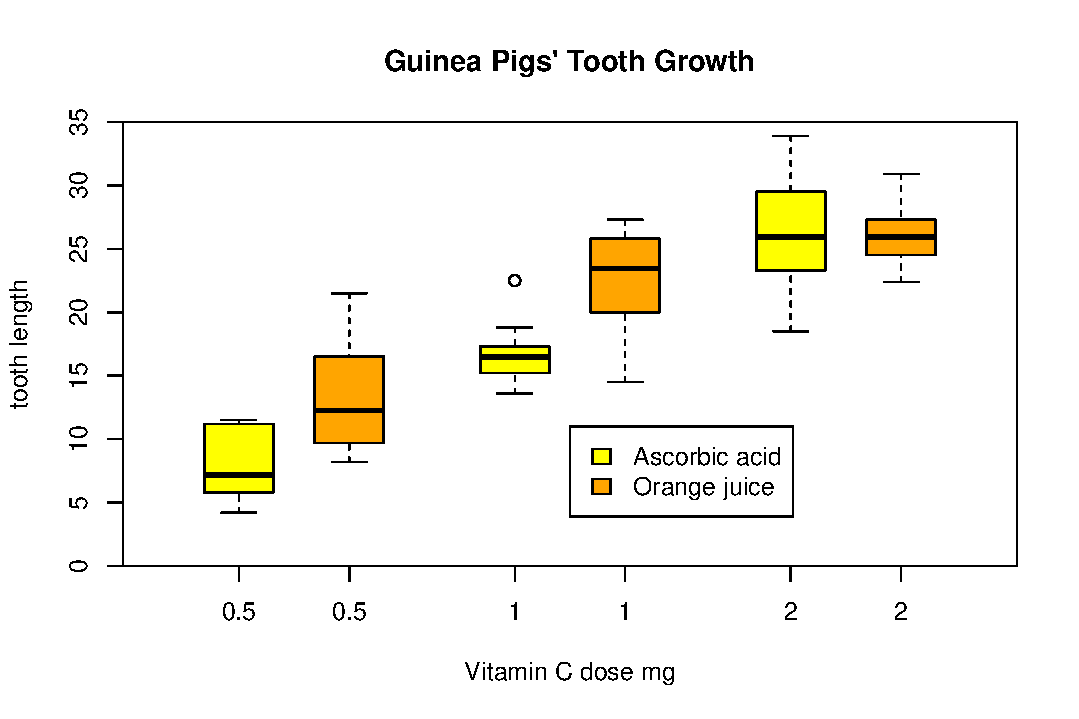
\includegraphics[width=4.8in, height=3.2in]{GuineaPigPlot.pdf}
\caption{Guinea pig tooth growth and vitamin C dose}
\label{fig:GPPlot}
\end{figure}

\subsection{Lists}
\begin{itemize}
\item Look before you leap
\item Then go for it
\item Enjoy the trip
\end{itemize}

This is a numbered list.
\begin{enumerate}
\item Frogs
\item Toads
\begin{enumerate}
\item Lesser spotted
\item Warty
\end{enumerate}
\end{enumerate}

\subsection{Maths}
This equation is part of the sentence: 
 $x\wedge (y\vee z) = (x\wedge y) \vee (x\wedge z)$ but the next one is
displayed separately.

$$\nabla^2 f(x,y) = \frac{\partial^2 f}{\partial x^2}
+ \frac{\partial^2 f}{\partial y^2}$$

\subsection{Tables}
A simple table

\begin{table}[htb]
\centering
\begin{tabular}{ll}
\textbf{Vegetables} & \textbf{Comments} \\
Carrots & Good early crop, then carrot fly. \\
French beans & Excellent.\\
\end{tabular}
\caption{Vegetable production}
\end{table}

\section{Conclusion}
Figure~\ref{fig:GPPlot} on page \pageref{fig:GPPlot} illustrates
the relationship between the amount of Vitamin C given and
their tooth growth \cite{Lamport}.

\clearpage
\section*{Appendix}
\begin{verbatim}
Put your R code here.
\end{verbatim}

\bibliographystyle{apalike2}

\bibliography{polygenic_bib}


\end{document}
